%!TEX root = ../dokumentation.tex

\section{Performance-Test}
\label{sec:Performance}
Um die Performance von \acs{Redis} zu testen, wurde der in \acs{Redis} integrierte Benchmark-Test verwendet.
Dieser kann einfach mit dem Befehl \textit{redis-benchmark} ausgeführt werden.
Dabei erreichte das System auf einem 2021er MacBook Air, ca. 180000 Schreiboperationen und über 200000 Leseoperationen pro Sekunde (vgl. \autoref{fig:redis-benchmark}).

\begin{figure}[H]
	\centering
	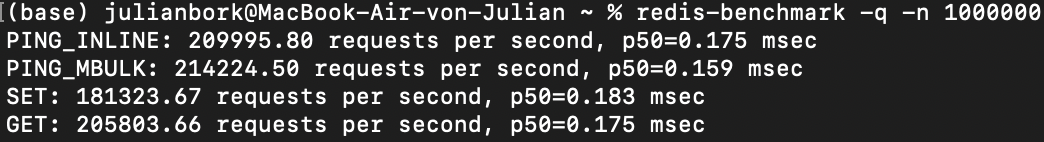
\includegraphics[width=0.8\textwidth]{images/redis-benchmark.png}
	\caption{Benchmark-Test}
	\label{fig:redis-benchmark}
\end{figure}

Hierbei ist zu beachten, dass die Geschwindigkeit der Datenbank sowohl von der benutzten Hardware als auch der Größe der Daten abhängt.
Besonders die CPU wird bei der Verarbeitung von Daten stark beansprucht. Da \acs{Redis} selbst allerdings nicht parallel arbeitet, ist die Anzahl der CPU-Kerne nicht ausschlaggebend für die Geschwindigkeit (vgl. \cite{Redis-Docs-Benchmarks}).

Dementsprechend ist es denkbar, dass die Geschwindigkeit mit potenterer Hardware, so wie sie in großen Serversystemen zum Einsatz kommt, noch weiter gesteigert werden kann.
